% Eğer Tezinizi bu dosyada yazacaksanız "TEZİNİZİ BURADAN SONRA EKLEYİNİZ" bölümünden sonra ekeleyebilirsiniz. Özet ve Summary bölümleri /bolum klasörünün içindedir.

\documentclass[]{esogu}			% Optionlar boş olacak, şablonu kullanmak için
\usepackage{lipsum}				% Örnek tezde anlamsız metin yazmak için bu paket gerekli. Tezinizde bu bölümü silebilirsiniz.
\usepackage{atbegshi} % İçindekiler, şekiller ve çizelgelerde birinci sayfadan sonraki sayfalara devam yazmak için
\makeatletter
\newcommand{\AtBeginShipoutClear}{\gdef\AtBegShi@Hook{}}
\makeatother
%\usepackage{glossaries}
\bibliography{kaynakca.bib}		% Kaynakça dosyası için Bunu Zotero, Mendeley, Endnote ya da CiteU gibi bir programla oluşturmanızı tavsiye ederim. Zotero hakkında bilgi http://makina.gmay.me/Bulutta/ adresindeki ekitapta mevcut.


%%%%%%%KISALTMALAR%%%%%%%%%%%%%%%%%%%
%% Kısaltmalar için lütfen glossaries paketine bakınız.
\newglossarystyle{mylong3col}{%
  \setglossarystyle{long3colheader}%
  \renewcommand\entryname{Simge veya Kısaltma}
  \renewcommand\descriptionname{Tanım}
  \renewcommand{\pagelistname}{Sayfa Numarası}
  \renewenvironment{theglossary}%
    {\begin{longtable}[l]{@{}lp{0.5\hsize}p{0.3\hsize}}}%
    {\end{longtable}}%
}


\printglossaries

\newacronym{OBEB}{OBEB}{Ortak Katların En Büyüğü}

\newacronym{SWD}{SWD}{Serial Write Debug}
\newacronym{OKEK}{OKEK}{Ortak Katların En Küçüğü}

\newacronym{pi}{$\pi$}{$\pi$ sayısı}

%----------------------------------------------------------------------------------------
\begin{document}

\frontmatter %roma rakamları ile yazdırmak için
\title{Pau Thesis}
%-----Dış kapak Türkçe---------- Burayı değiştirmeyin
\begin{titlingpage*}
\begin{center}
\large
\textbf{\MakeUppercase{\uni}}

\vspace{1pc}
\textbf{\MakeUppercase{\fakulte}}

\vspace{1pc}
\textbf{\MakeUppercase{\bolum}}
\vspace{2pc}

%---------------bolum logosu-------------------------
	\begin{figure}[h]
	\centering
	
\includegraphics[width=0.25\textwidth]{gorseller/image1}
	\end{figure}
	\vspace{2pc}
  \Large
	\textbf{\unvan\space BİTİRME TEZİ}\\
  \vspace{1pc}							%12 punto boşluk ver
  \normalsize
\end{center}
\begin{framed}
\begin{center}
\textbf{GÜÇ ELEKTRONİĞİ TABANLI \\MİKROİŞLEMCİLERİN PROGRAMLANMASI\\ VE VERİ AKTARIMI} %Daha toplu olmasi icin boyle yaptim
\vspace{1pc}

\yazar\\
\vspace{1pc}

\teslim\\
\vspace{1pc}

Tez Danışmanı:\hspace{10mm} \danisman
\end{center}
\end{framed}
\end{titlingpage*}

%---------------Tez kunyesi-----------------------

\begin{table}[]
\begin{tabular}{|l|l|}
\hline
\multicolumn{2}{|c|}{\textbf{TEZ KÜNYESİ}}      \\ \hline
1. ARŞİV NUMARASI    & 2. SAVUNMA TARİHİ \\
\hspace{10ex}       & \hspace{2ex}5 Eylül 2018    \\ \hline
\multicolumn{2}{|l|}{4.TEZ BAŞLIĞI}    \\
\multicolumn{2}{|p{14cm}|}{\hspace{2ex}\tbaslik}\\ \hline
5.YAZAR              & 6.TEZ DANIŞMANI \\
\hspace{2ex}\yazar   & \hspace{2ex}\danisman  \\ \hline
\multicolumn{2}{|l|}{6.ÖZET}           \\
\multicolumn{2}{|p{14cm}|}{\hangindent=2ex\hspace{2ex}\lipsum[1]}              \\ \hline
7.ANAHTAR KELİMELER & 8.SAYFA SAYISI   \\
\hspace{10pt}             & \hspace{10pt}  \\ \hline
\end{tabular}
\end{table}

\clearpage
%----------Onay-------------------------------------
\thispagestyle{empty}
\begin{center}
\large
\textbf{\MakeUppercase{\tbaslik}}\\
\vspace{1pc}
\yazar\\
\vspace{1pc}
\teslim\\
\vspace{2pc}
\end{center}
\vspace{2pc}
\normalsize
Bu çalışma, jürimiz tarafından Elektrik-Elektronik Mühendisliği Bölümü’nde Lisans
Bitirme Tezi olarak kabul edilmiştir.

\vspace{20mm}

\noindent \textbf{Tez Danışmanı:\hspace{5ex}\danisman}

\hspace{20ex}\uni

\hspace{20ex}\fakulte

\hspace{20ex}\bolum
\vspace{1pc}

\noindent \textbf{Üye:\hspace{15ex}\jbir}

\hspace{20ex}\uni

\hspace{20ex}\fakulte

\hspace{20ex}\bolum
\vspace{1ex}

\noindent \textbf{Üye:\hspace{15ex}\jiki}

\hspace{20ex}\uni

\hspace{20ex}\fakulte

\hspace{20ex}\bolum
\vspace{1pc}

\noindent \textbf{Onaylayan:\hspace{9ex}\onay}

\hspace{20ex}\uni

\hspace{20ex}\fakulte

\hspace{20ex}\bolum
\newpage


%-------------------Şekiller ve Çizelgeler Dizini----------------
\renewcommand{\listfigurename}{ŞEKİLLER LİSTESİ}
\renewcommand{\listtablename}{TABLOLAR LİSTESİ}

\setlength\beforechapskip{-\baselineskip}

\normalsize

%Özette tez çalışmasının amacı, kapsamı, kullanılan yöntemler ve varılan sonuçlar açık ve öz olarak belirtilmeli, bunlar alt başlıklar altında sunulmamalıdır.  Özetin uzunluğu 250 kelimeyi geçmemelidir. 

%Summary sayfasının içeriği ve düzeni tümüyle Özet sayfasının aynı olmalı ve (vii) ile numaralanmalıdır.

%Özet ve Summary’nin altına anahtar kelimeler/keywords yazılmalıdır.  Konu literatürde hangi kelimelerle geçiyorsa anahtar kelime olarak bu kelimeler kullanılmalıdır.

\chapter{ÖZET}

\lipsum[1]
\chapter{SUMMARY}
\lipsum[1-2]
\chapter{TEŞEKKÜR}

Öncelikle, yetişmemde en büyük pay sahibi olan aileme teşekkür etmeyi bir vazife olarak görüyorum.
Bu çalışma süresince beni yönlendiren ve yardımlarını benden esirgemeyen tez danışmanım sayın Doç. Dr. Selami Kesler'e teşekkürlerimi sunarım. Ayrıca tez çalışmamı hazırlamamda, çeşitli konularda yardımlarından dolayı Abdülkadir ABAKAY'a ve Raşit EVDÜZEN'e teşekkürlerimi sunarım.
\\\\\\
\textbf{Çağatay YILMAZ}


\AtBeginShipout{\protect\chapter*{İÇİNDEKİLER (Devam)}}
\tableofcontents*
\AtBeginShipoutClear
\newpage
\AtBeginShipout{\protect\chapter*{ŞEKİLLER LİSTESİ (Devam)}}
\listoffigures
\AtBeginShipoutClear
\newpage
\AtBeginShipout{\protect\chapter*{ÇİZELGELER LİSTESİ (Devam)}}
\listoftables
\AtBeginShipoutClear
\clearpage

\clearpage
\printglossary[style=mylong3col, type=\acronymtype, title=Simgeler ve Kısaltmalar Listesi, toctitle=SİMGELER VE KISALTMALAR LİSTESİ]
\clearpage


\mainmatter %arap harfleri ile yazdırmak için
% AltBölüm numaralaması
\setcounter{secnumdepth}{5} % 5 derine kadar numara ver.
%---------TEZİNİZİ BURADAN SONRA EKLEYİNİZ-----------------



\chapter{GİRİŞ}

Güç elektroniği serüvenine 1900'lü yıllarda güç elektroniği doğru akım motorlarının hız kontrolü ile başlamıştır.
Elektron tüpleri ile teorik çalışmalar yapılmıştır, fakat uygulamaya sokulmamıştır.
1950 yılında yarıiletkenler, 1960 yılında tristörler, 1980 yılında sayısal elektronik ve
mikroişlemcilerin geliştirilmesi ile güç elektroniği otomotiv, endüstri, ulaşım araçları gibi bir çok sektörde faailiyet
göstermektedir.

Güç elektroniğinde mikrodenetleyiciler, yarıiletkelerin ihtiyaç duyduğu tetikleme sinyallerinin oluştrulması,
akım ve gerilim değerlerin okunması gibi ihtiyaçları karşılmaktadır.

İletişim altyapısını ve teknik gelişmeler sonucu günümüzün popüler konusu olan nesnelerin interneti ile,
güç elektroniği uygulamarında kullananılan mikrodenetleyicilerin uzaktan erişim ile yazılımlarının ve paremetrelerinin
güncellenmesi, denetleyici tarafıdan okunan değerlerin görüntülenmesi gibi ihtiyaçlar ortaya çıkmıştır.

Bu çalışmada belirtilen ihtiyaçları karşılamak amacıyla; güç elektroniğinde sıklıkla kullanılan ARM tabanlı mikrodenetleyiciler
için programlamama ve veri aktarımı sağlamak üzere ESP8266 mikroişlemcisi kullanıldı.
ESP8266 hedef denetleyicinin debug portu olan \acrfull{SWD} portuna bağlı olacak ve buradan işemcinin
registerlarına ve hafıza birimlerine erişecek. Aynı zamanda web server olarak çalışacak ve kullanıcı ile hedef
işlemci arasında arayüz oluşturacaktır.



				% Metni dosyadan çağırmak için örnek
\chapter{LİTERATÜR ARAŞTIRMASI}

Basit iki terimle \acrfull{OBEB} ve \acrfull{OKEK} kısaltmaları anlatabiliriz. İster kısaltmasını \acrshort{OBEB}, isterseniz de uzun açılımını \acrlong{OKEK} yazdırabilirsiniz. Bunu yapabilmek için dosyanın başında terimleri tanımlamanız gereklidir. İsterseniz matematik terimlerini de, örneğin \acrshort{pi} böyle tanımlayabilirsiniz. Uzun uzun \acrfull{pi} yazmanız gerekmez. 

Teorem yazmak isterseniz:
\begin{theorem}[Öklid]
 İki noktadan bir ve yalnız bir doğru geçer.
\end{theorem}

İspat yazmak isterseniz:
\begin{ispat}[Tezin en önemli ispatı]
x=10
\end{ispat}
\lipsum[1-2]
\begin{figure}[h]
\centering
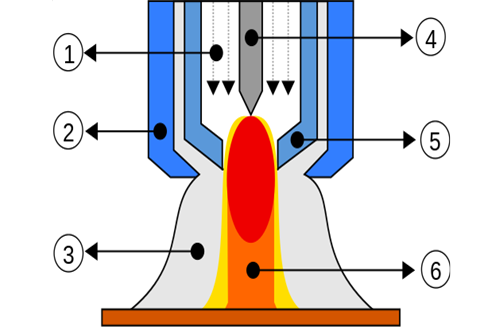
\includegraphics[width=\textwidth]{gorseller/ptaTorc}
\caption{PTA Torç}\label{fig:PtaTorc1}
\end{figure}
\lipsum[1-2]
\begin{table}
\centering
\caption{Deneme Tablosu.}\label{tab:den1}
\begin{tabular}{|l|l|l|}
\hline
sıra   & sayı   & toplam \\ \hline
1      & 2      & 3      \\ \hline
Kelime & deneme & son    \\ \hline
\end{tabular}
\end{table}


\section{Literatür Araştırması Birinci Derece Başlık}
\lipsum[1-2]
\begin{figure}[h]
\centering
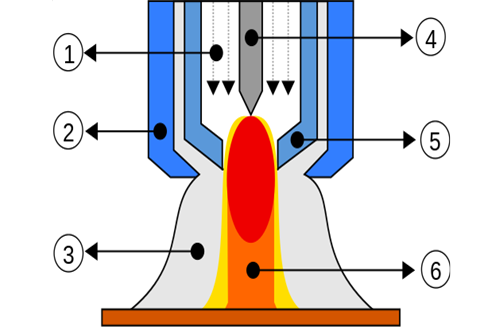
\includegraphics[width=\textwidth]{gorseller/ptaTorc}
\caption{PTA Torç}\label{fig:PtaTorc1}
\end{figure}
\lipsum[1-2]
\begin{table}
\centering
\caption{Deneme Tablosu.}\label{tab:den1}
\begin{tabular}{|l|l|l|}
\hline
sıra   & sayı   & toplam \\ \hline
1      & 2      & 3      \\ \hline
Kelime & deneme & son    \\ \hline
\end{tabular}
\end{table}
Teorem yazmak isterseniz:
\begin{theorem}[Öklid]
 İki noktadan bir ve yalnız bir doğru geçer.
\end{theorem}

İspat yazmak isterseniz:
\begin{ispat}[Tezin en önemli ispatı]
x=10
\end{ispat}

\subsection{Literatür Araştırması ikinci derece başlık}
\lipsum[1-2]
\begin{figure}[h]
\centering
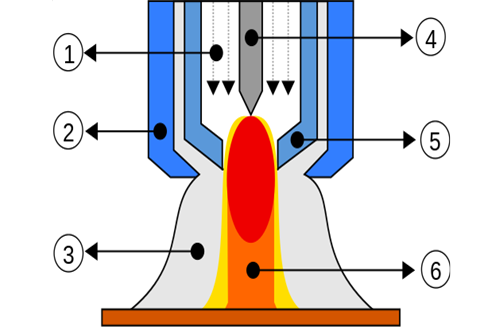
\includegraphics[width=\textwidth]{gorseller/ptaTorc}
\caption{PTA Torç}\label{fig:PtaTorc1}
\end{figure}
\lipsum[1-2]
\begin{table}
\centering
\caption{Deneme Tablosu.}\label{tab:den1}
\begin{tabular}{|l|l|l|}
\hline
sıra   & sayı   & toplam \\ \hline
1      & 2      & 3      \\ \hline
Kelime & deneme & son    \\ \hline
\end{tabular}
\end{table}

Teorem yazmak isterseniz:
\begin{theorem}[Öklid]
 İki noktadan bir ve yalnız bir doğru geçer.
\end{theorem}

İspat yazmak isterseniz:
\begin{ispat}[Tezin en önemli ispatı]
x=10
\end{ispat}

\subsubsection{Literatür araştırması dördüncü derece başlık}
\lipsum[1-2]
\begin{figure}[h]
\centering
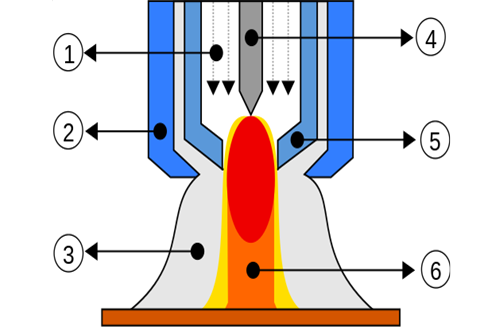
\includegraphics[width=\textwidth]{gorseller/ptaTorc}
\caption{PTA Torç}\label{fig:PtaTorc1}
\end{figure}
\lipsum[1-2]
\begin{table}
\centering
\caption{Deneme Tablosu.}\label{tab:den1}
\begin{tabular}{|l|l|l|}
\hline
sıra   & sayı   & toplam \\ \hline
1      & 2      & 3      \\ \hline
Kelime & deneme & son    \\ \hline
\end{tabular}
\end{table}

Teorem yazmak isterseniz:
\begin{theorem}[Öklid]
 İki noktadan bir ve yalnız bir doğru geçer.
\end{theorem}

İspat yazmak isterseniz:
\begin{ispat}[Tezin en önemli ispatı]
x=10
\end{ispat}
\chapter{BULGULAR VE TARTIŞMA}

Basit iki terimle \acrfull{OBEB} ve \acrfull{OKEK} kısaltmaları anlatabiliriz. İster kısaltmasını \acrshort{OBEB}, isterseniz de uzun açılımını \acrlong{OKEK} yazdırabilirsiniz. Bunu yapabilmek için dosyanın başında terimleri tanımlamanız gereklidir. İsterseniz matematik terimlerini de, örneğin \acrshort{pi} böyle tanımlayabilirsiniz. Uzun uzun \acrfull{pi} yazmanız gerekmez. 

Teorem yazmak isterseniz:
\begin{theorem}[Öklid]
 İki noktadan bir ve yalnız bir doğru geçer.
\end{theorem}

İspat yazmak isterseniz:
\begin{ispat}[Tezin en önemli ispatı]
x=10
\end{ispat}
\lipsum[1-2]
\begin{figure}[h]
\centering
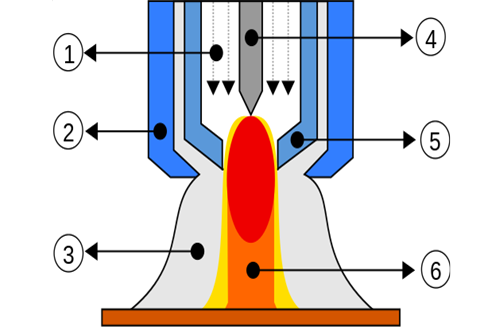
\includegraphics[width=\textwidth]{gorseller/ptaTorc}
\caption{PTA Torç}\label{fig:PtaTorc1}
\end{figure}
\lipsum[1-2]
\begin{table}
\centering
\caption{Deneme Tablosu.}\label{tab:den1}
\begin{tabular}{|l|l|l|}
\hline
sıra   & sayı   & toplam \\ \hline
1      & 2      & 3      \\ \hline
Kelime & deneme & son    \\ \hline
\end{tabular}
\end{table}


\section{Bulgular ve Tartışma Birinci Derece Başlık}
\lipsum[1-2]
\begin{figure}[h]
\centering
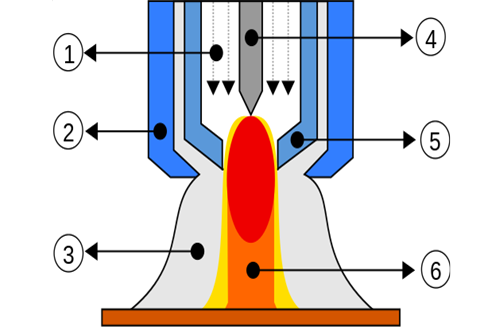
\includegraphics[width=\textwidth]{gorseller/ptaTorc}
\caption{PTA Torç}\label{fig:PtaTorc1}
\end{figure}
\lipsum[1-2]
\begin{table}
\centering
\caption{Deneme Tablosu.}\label{tab:den1}
\begin{tabular}{|l|l|l|}
\hline
sıra   & sayı   & toplam \\ \hline
1      & 2      & 3      \\ \hline
Kelime & deneme & son    \\ \hline
\end{tabular}
\end{table}
Teorem yazmak isterseniz:
\begin{theorem}[Öklid]
 İki noktadan bir ve yalnız bir doğru geçer.
\end{theorem}

İspat yazmak isterseniz:
\begin{ispat}[Tezin en önemli ispatı]
x=10
\end{ispat}

\subsection{Bulgular ve Tartışma ikinci derece başlık}
\lipsum[1-2]
\begin{figure}[h]
\centering
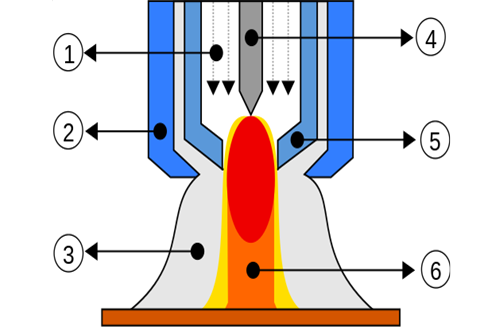
\includegraphics[width=\textwidth]{gorseller/ptaTorc}
\caption{PTA Torç}\label{fig:PtaTorc1}
\end{figure}
\lipsum[1-2]
\begin{table}
\centering
\caption{Deneme Tablosu.}\label{tab:den1}
\begin{tabular}{|l|l|l|}
\hline
sıra   & sayı   & toplam \\ \hline
1      & 2      & 3      \\ \hline
Kelime & deneme & son    \\ \hline
\end{tabular}
\end{table}

Teorem yazmak isterseniz:
\begin{theorem}[Öklid]
 İki noktadan bir ve yalnız bir doğru geçer.
\end{theorem}

İspat yazmak isterseniz:
\begin{ispat}[Tezin en önemli ispatı]
x=10
\end{ispat}

\subsubsection{Bulgular ve tartışma dördüncü derece başlık}
\lipsum[1-2]
\begin{figure}[h]
\centering
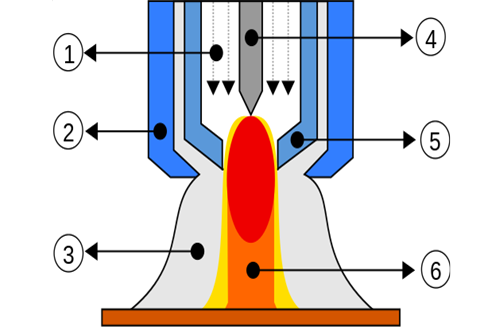
\includegraphics[width=\textwidth]{gorseller/ptaTorc}
\caption{PTA Torç}\label{fig:PtaTorc1}
\end{figure}
\lipsum[1-2]
\begin{table}
\centering
\caption{Deneme Tablosu.}\label{tab:den1}
\begin{tabular}{|l|l|l|}
\hline
sıra   & sayı   & toplam \\ \hline
1      & 2      & 3      \\ \hline
Kelime & deneme & son    \\ \hline
\end{tabular}
\end{table}

Teorem yazmak isterseniz:
\begin{theorem}[Öklid]
 İki noktadan bir ve yalnız bir doğru geçer.
\end{theorem}

İspat yazmak isterseniz:
\begin{ispat}[Tezin en önemli ispatı]
x=10
\end{ispat}
Eğer metin içinde \(\lim_{x \to \infty} \exp(-x) = 0\) ya da ortalayabilir
\begin{displaymath}
\cos (2\theta) = \cos^2 \theta - \sin^2 \theta
\end{displaymath}
isterseniz de numaralı denklem yazabilirsiniz.

\begin{equation}
\frac{\mathrm d}{\mathrm d x} \left( k g(x) \right)
\end{equation}
\subsubsection{Kimya}
\ce{B4C} yazabilirsiniz. Ya da

\ce{CO2 + C -> 2CO}

Daha fazlası için mhchem paketine bakınız.
 
\section{Analiz}
Eğer metin içinde şekile referans vermek isterseniz Şekil\ref{fig:PtaTorc} yazarsınız. 

Kaynakça böyle verilebilir \parencite{celik_microstructure_2013} ya da iki yazarlı ise böyle verilebilir \parencite{gatto_plasma_2004} veya ikiden fazla ise böyle verilebilir.
\parencite{celik_effects_2011}

Kaynakça listesi için daha çok referans verilmek istenirse \parencite{yazdi_microstructure_2015, keehan_influence_2006, guo_microstructure_2014}, \parencite{kim_variation_2013}, bir başkası \parencite{xibao_metallurgical_2005},  ya da başkası \parencite{jin_effect_1997} kullanılabilir.
\chapter{SONUÇLAR VE ÖNERİLER}

Basit iki terimle \acrfull{OBEB} ve \acrfull{OKEK} kısaltmaları anlatabiliriz. İster kısaltmasını \acrshort{OBEB}, isterseniz de uzun açılımını \acrlong{OKEK} yazdırabilirsiniz. Bunu yapabilmek için dosyanın başında terimleri tanımlamanız gereklidir. İsterseniz matematik terimlerini de, örneğin \acrshort{pi} böyle tanımlayabilirsiniz. Uzun uzun \acrfull{pi} yazmanız gerekmez. 

Teorem yazmak isterseniz:
\begin{theorem}[Öklid]
 İki noktadan bir ve yalnız bir doğru geçer.
\end{theorem}

İspat yazmak isterseniz:
\begin{ispat}[Tezin en önemli ispatı]
x=10
\end{ispat}
\lipsum[1-2]
\begin{figure}[h]
\centering
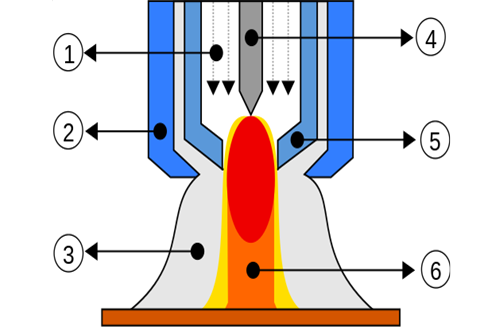
\includegraphics[width=\textwidth]{gorseller/ptaTorc}
\caption{PTA Torç}\label{fig:PtaTorc1}
\end{figure}
\lipsum[1-2]
\begin{table}
\centering
\caption{Deneme Tablosu.}\label{tab:den1}
\begin{tabular}{|l|l|l|}
\hline
sıra   & sayı   & toplam \\ \hline
1      & 2      & 3      \\ \hline
Kelime & deneme & son    \\ \hline
\end{tabular}
\end{table}


\section{Sonuçlar ve Öneriler Birinci Derece Başlık}
\lipsum[1-2]
\begin{figure}[h]
\centering
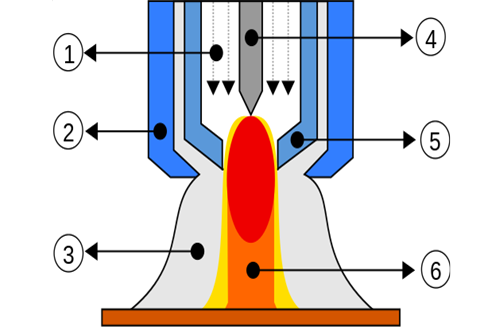
\includegraphics[width=\textwidth]{gorseller/ptaTorc}
\caption{PTA Torç}\label{fig:PtaTorc1}
\end{figure}
\lipsum[1-2]
\begin{table}
\centering
\caption{Deneme Tablosu.}\label{tab:den1}
\begin{tabular}{|l|l|l|}
\hline
sıra   & sayı   & toplam \\ \hline
1      & 2      & 3      \\ \hline
Kelime & deneme & son    \\ \hline
\end{tabular}
\end{table}
Teorem yazmak isterseniz:
\begin{theorem}[Öklid]
 İki noktadan bir ve yalnız bir doğru geçer.
\end{theorem}

İspat yazmak isterseniz:
\begin{ispat}[Tezin en önemli ispatı]
x=10
\end{ispat}

\subsection{Sonuçlar ve Öneriler ikinci derece başlık}
\lipsum[1-2]
\begin{figure}[h]
\centering
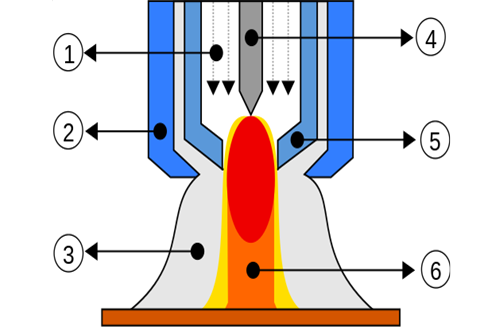
\includegraphics[width=\textwidth]{gorseller/ptaTorc}
\caption{PTA Torç}\label{fig:PtaTorc1}
\end{figure}
\lipsum[1-2]
\begin{table}
\centering
\caption{Deneme Tablosu.}\label{tab:den1}
\begin{tabular}{|l|l|l|}
\hline
sıra   & sayı   & toplam \\ \hline
1      & 2      & 3      \\ \hline
Kelime & deneme & son    \\ \hline
\end{tabular}
\end{table}

Teorem yazmak isterseniz:
\begin{theorem}[Öklid]
 İki noktadan bir ve yalnız bir doğru geçer.
\end{theorem}

İspat yazmak isterseniz:
\begin{ispat}[Tezin en önemli ispatı]
x=10
\end{ispat}

\subsubsection{Sonuçlar ve Öneriler dördüncü derece başlık}
\lipsum[1-2]
\begin{figure}[h]
\centering
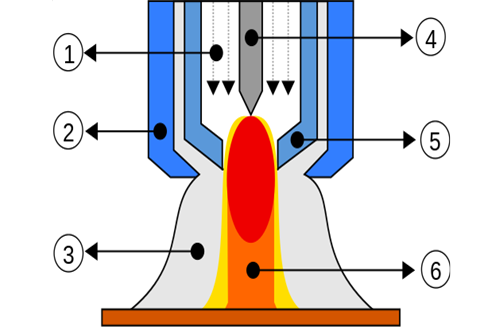
\includegraphics[width=\textwidth]{gorseller/ptaTorc}
\caption{PTA Torç}\label{fig:PtaTorc1}
\end{figure}
\lipsum[1-2]
\begin{table}
\centering
\caption{Deneme Tablosu.}\label{tab:den1}
\begin{tabular}{|l|l|l|}
\hline
sıra   & sayı   & toplam \\ \hline
1      & 2      & 3      \\ \hline
Kelime & deneme & son    \\ \hline
\end{tabular}
\end{table}

Teorem yazmak isterseniz:
\begin{theorem}[Öklid]
 İki noktadan bir ve yalnız bir doğru geçer.
\end{theorem}

İspat yazmak isterseniz:
\begin{ispat}[Tezin en önemli ispatı]
x=10
\end{ispat}

\newpage

\printbibliography[title={KAYNAKLAR\space DİZİNİ}] %numaralı olsun istersen optionlarda heading=bibnumbered, yaz
\defbibheading{bibliography}[\refname]{%
  \section*{#1}%
  \markboth{\MakeUppercase{#1}}{\MakeUppercase{#1}}}

\addcontentsline{toc}{chapter}{\textbf{Özgeçmiş}}   % Sadece doktora tezleri için

\end{document}
